\documentclass{beamer}
\usepackage[utf8x]{inputenc}
\usepackage{hyperref}
\usepackage[footheight=1em]{beamerthemeboxes}
%\usepackage{pgfpages}
%\setbeameroption{show notes on second screen=left}
\usetheme{Singapore}

%\usetheme{Frankfurt}


%\addfootboxtemplate{\color{white}}{\color{gray}
  %\insertframenumber/\inserttotalframenumber\null}



%\setbeamertemplate{background canvas}{\includegraphics
%   [width=\paperwidth,height=\paperheight]{img/fond.png}}


\title{Implémentation de l'algorithme de Dinic et d'Edmonds-Karp}
\subtitle{TP Algorithmique, Complexité \& Calculabilité (FMIN105)}
\author{William Dyce \and Thibaut Marmin \\ Clément Sipieter}
\institute{Université Montpellier 2\\Encadré par Rodolphe Giroudeau}
\date{15 Décembre 2011}

\begin{document}

\AtBeginSection[]
{
  \begin{frame}{TP Algorithmique, Complexité \& Calculabilité}
  \begin{columns}[t]
  \begin{column}{5cm}
  \tableofcontents[sections={1-3},currentsection,hideothersubsections]
  \end{column}
  \begin{column}{5cm}
  \tableofcontents[sections={4-6},currentsection,hideothersubsections]
  \end{column}
  \end{columns}
  \end{frame}
}

\begin{frame}
\titlepage
\end{frame}

\begin{frame}{TP Algorithmique, Complexité \& Calculabilité}
    

  \begin{columns}[t]
  \begin{column}{5cm}
  \tableofcontents[sections={1-3},hideallsubsections]
  \end{column}
  \begin{column}{5cm}
  \tableofcontents[sections={4-6},hideallsubsections]
  \end{column}
  \end{columns}

\end{frame}

\section{Présentation du sujet}
\subsection{Algorithmes}
\begin{frame}{Algorithmes}{Ford-Fulkerson : $O(mnC^*)$}

\begin{block}{Idée générale}
\begin{itemize}
\item Trouver une chaîne améliorante.
\item Augmenter le flot le long de cette chaîne.
\end{itemize}
\end{block}

\begin{block}{Faiblesses}
\begin{itemize}
\item "Pseudo-exponentielle" : $O(n^3)$, mais seulement pour des capacités bornées \ldots
\item "Diamant maudit" : $2\times{M}$ itérations! 
\end{itemize}
\end{block}
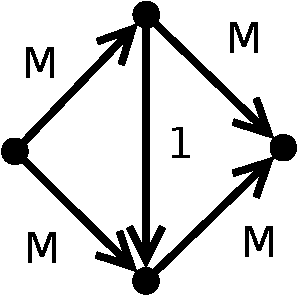
\includegraphics[width=0.3\textwidth]{img/maudit}

\end{frame}
\begin{frame}{Algorithmes}{Edmonds-Karp : $O(n^2m)$}

\begin{block}{Idée générale}
\begin{itemize}
\item Prendre la chaîne la plus courte en nombre d'arcs
\end{itemize}
\end{block}

\begin{block}{Faiblesses}
\begin{itemize}
\item Graphes avec de multiples chemins de plus en plus longs \dots
\end{itemize}
\end{block}
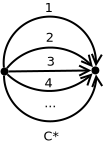
\includegraphics[width=0.3\textwidth]{img/anti_ek}

\end{frame}

\begin{frame}{Algorithmes}{Dinic : $O(nm^2)$}
\begin{block}{Idée générale}
\begin{itemize}
\item Rechercher un ensemble de chemins à la fois
\item Trouver un "Flot Bloquant" dans le "Graphe de Couches"
\end{itemize}
\end{block}
\end{frame}

\section{Implémentation}
\subsection{Présentation générale}
\begin{frame}{Implémentation}{Présentation générale}
\begin{itemize}
\item Choix du langage
\item Choix d'implémentation
\item Etc\ldots
\end{itemize}
\end{frame}

\subsection{Diagramme de classes}
\begin{frame}{Implémentation}{Diagramme de classes}
\end{frame}

\subsection{Structures de données}
\begin{frame}{Implémentation}{Structures de données}
\end{frame}

\subsection{Génération de graphes aléatoires}
\begin{frame}{Implémentation}{Génération de graphes aléatoires}
\end{frame}


\subsection{Fonctionnement général}
\begin{frame}{Implémentation}{Fonctionnement général}
\end{frame}

\section{Tests \& résultats}
\subsection{Méthode de tests}
\begin{frame}{Méthode de tests}{Série de tests}
\begin{block}{Complexité}
  \begin{itemize}
    \item Edmonds-Karp : $O(nm^2)$
    \item Dinic : $O(n^2m)$
  \end{itemize}
\end{block}
\begin{block}{Tests effectués}
  \begin{itemize}
    \item Nombre de sommets : 100, 200, 300, \ldots 1000
    \item Densité du graphe : 20\%, 50\% et 80\%
  \end{itemize}
\end{block}
\end{frame}

\begin{frame}{Méthode de tests}{Profiling}
\begin{block}{GNU gprof}
Profiler, analyse du code en fonction du temps passé par chaque fonction à l’exécution.
\begin{itemize}
\item Compilation avec l'argument \texttt{-pg}
\item Exécution du programme, génération du fichier \texttt{gmon.out}
\item Exportation des statistiques en fichier texte
\end{itemize}
\end{block}
\end{frame}

\begin{frame}{Tests \& résultats}{Profiling}
\begin{block}{GNU gprof}
Statistique fournies pour chaque fonction :
\begin{itemize}
\item \% temps cpu total
\item temps cpu
\item temps cpu par appel (de manière cumulative ou non)
\end{itemize}
\end{block}
\end{frame}

\subsection{Résultats}
\begin{frame}{Résultats}
\begin{center}
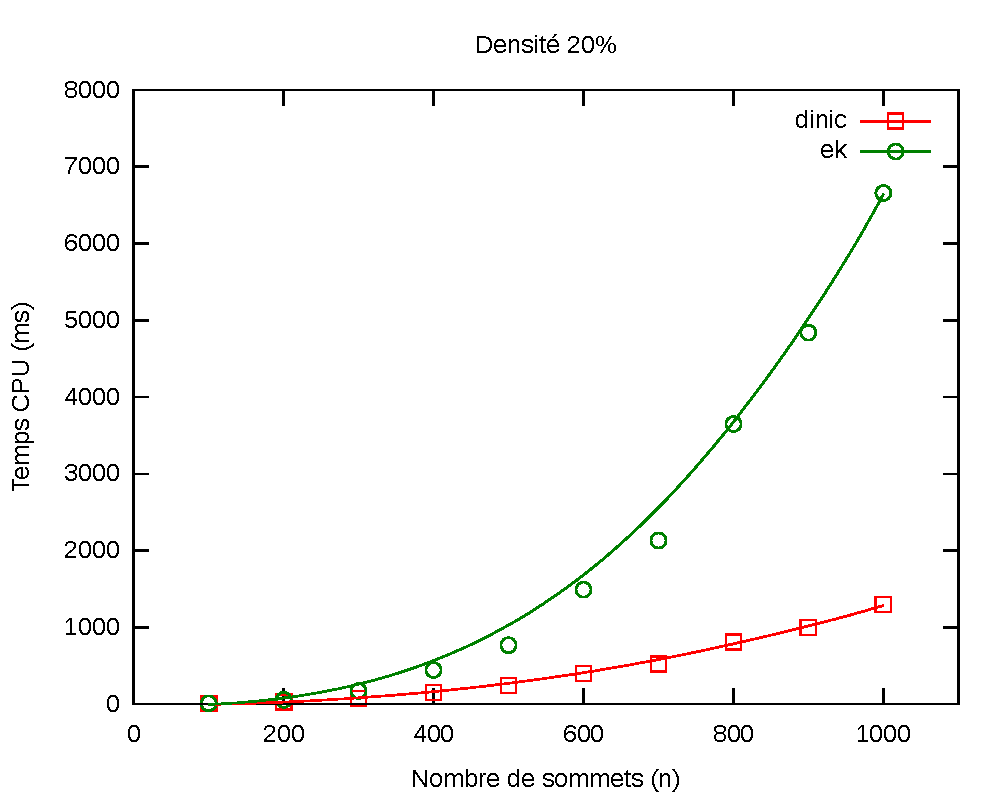
\includegraphics[width=0.8\textwidth]{img/c20}
\end{center}
\end{frame}
\begin{frame}{Résultats}
\begin{center}
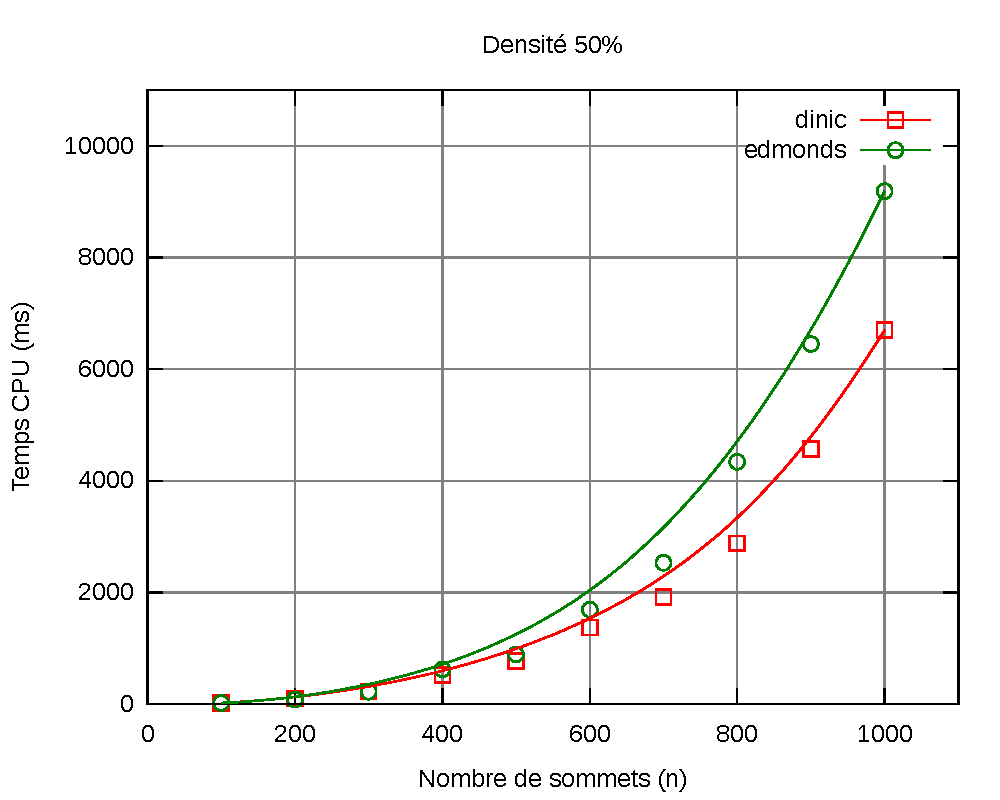
\includegraphics[width=0.8\textwidth]{img/c50}
\end{center}
\end{frame}
\begin{frame}{Résultats}
\begin{center}
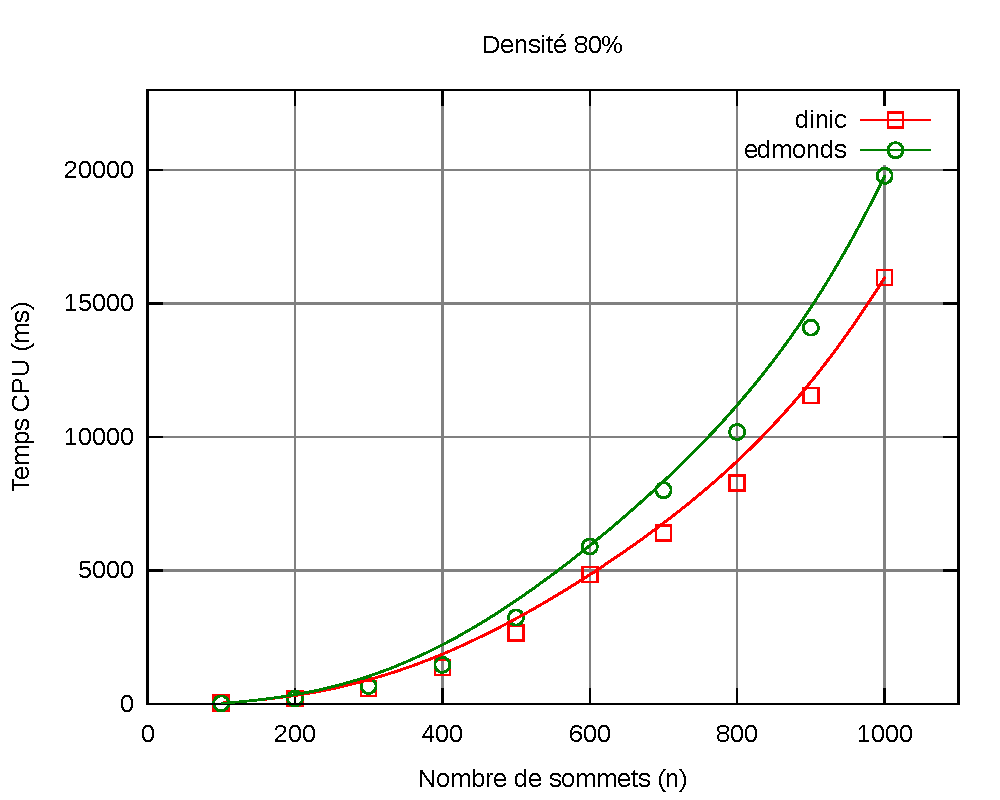
\includegraphics[width=0.8\textwidth]{img/c80}
\end{center}
\end{frame}
\begin{frame}{Résultats}
\begin{center}
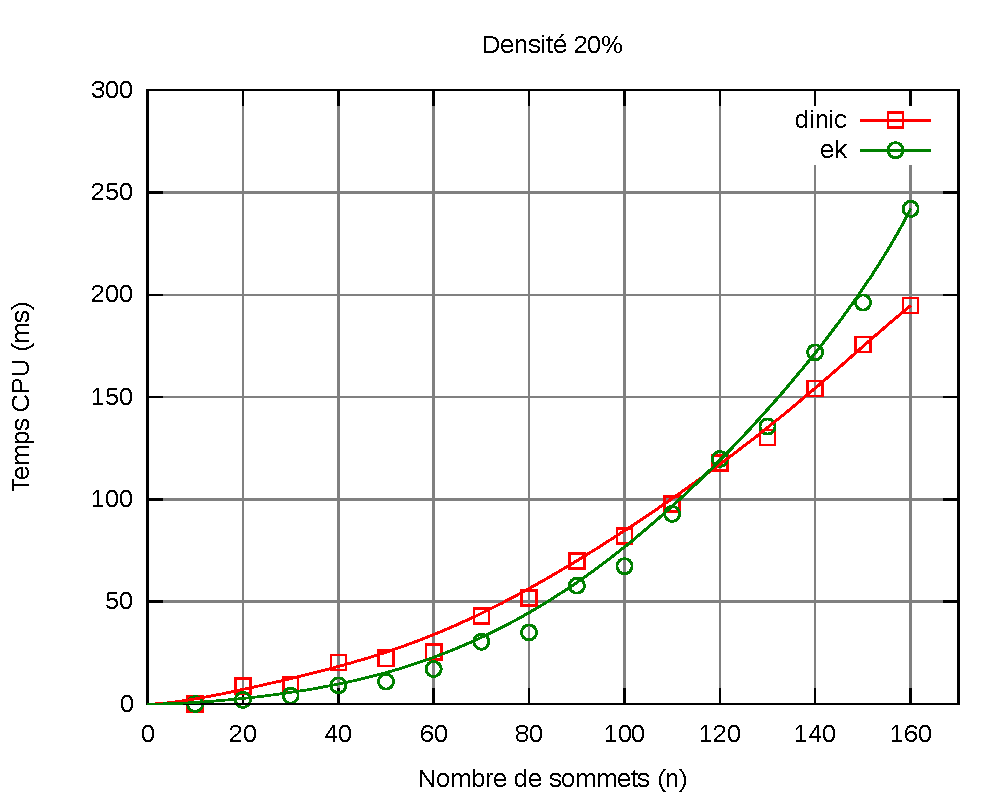
\includegraphics[width=0.8\textwidth]{img/c20_low}
\end{center}
\end{frame}
\begin{frame}{Résultats}
\begin{center}
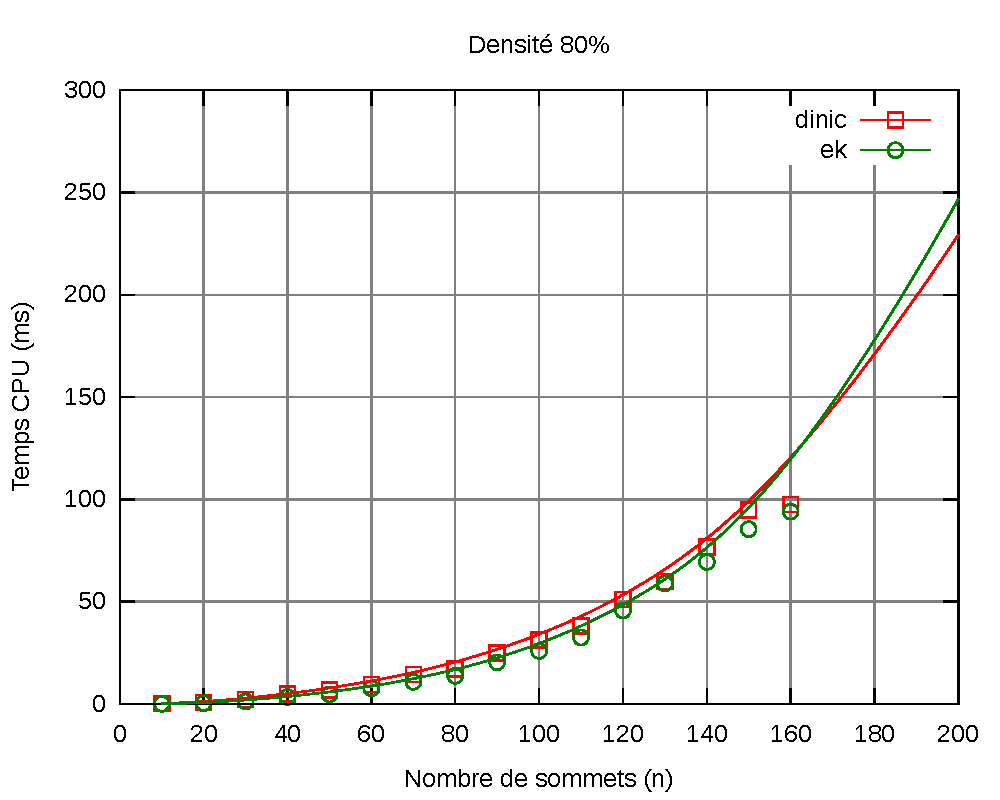
\includegraphics[width=0.8\textwidth]{img/c80_low}
\end{center}
\end{frame}
\begin{frame}{Résultats}{Conclusion}
\begin{itemize}
\item Dinic globalement plus rapide
\item Surtout sur des graphes peu denses
\item Edmonds-Karp efficace sur des petits graphes
\end{itemize}
$\Rightarrow$ Cohérence avec les complexités théoriques
\begin{center}
\begin{tabular}{ccc}
&$\swarrow\ \ \ \ \ \ \searrow$&\\
Dinic&&Edmonds-Karp\\
$O(nm^2)$&&$O(n^2m)$
\end{tabular}
\end{center}
\end{frame}

\section{Conclusion}
\subsection{Conclusion}
\begin{frame}{Conclusion}

\end{frame}

\section{Démonstration}
\subsection{Démonstration}
\begin{frame}{Démonstration}

\end{frame}

\end{document}